\subsection{The Big Oh Notation}

\begin{figure}[H]
  \centering
     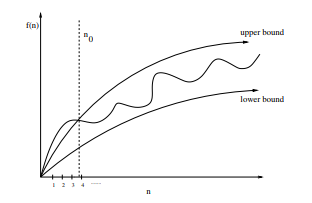
\includegraphics[scale=0.6]{./2_2.png}
  \label{fig:demo-diagram2-2}
  \caption{Upper and lower bounds valid for n>n0 smooth out the behavior of complex
		   functions}
\end{figure}

\begin{figure}[H]
  \centering
     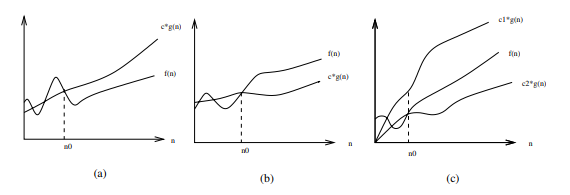
\includegraphics[scale=0.6]{./2_3.png}
  \label{fig:demo-diagram2-3}
  \caption{ Illustrating the big (a) O, (b) $\Omega$, and (c) $\Theta$ notations}
\end{figure}

\textbf{Stop and Think: Hip to the Squares} \\

\emph{Problem: Is $(x+y)^{2} = O(x^{2} + y^{2})$}

\noindent\rule{\textwidth}{0.4pt}

\textbf{Stop and Think: Back to the Definition} \\

\emph{Problem: Is $2^{n+1} = \Theta (2^{n}) ?$}

\noindent\rule{\textwidth}{0.4pt}